\documentclass[11pt,preprint]{elsarticle}

\usepackage{lmodern}
%%%% My spacing
\usepackage{setspace}
\setstretch{1.2}
\DeclareMathSizes{12}{14}{10}{10}

% Wrap around which gives all figures included the [H] command, or places it "here". This can be tedious to code in Rmarkdown.
\usepackage{float}
\let\origfigure\figure
\let\endorigfigure\endfigure
\renewenvironment{figure}[1][2] {
    \expandafter\origfigure\expandafter[H]
} {
    \endorigfigure
}

\let\origtable\table
\let\endorigtable\endtable
\renewenvironment{table}[1][2] {
    \expandafter\origtable\expandafter[H]
} {
    \endorigtable
}


\usepackage{ifxetex,ifluatex}
\usepackage{fixltx2e} % provides \textsubscript
\ifnum 0\ifxetex 1\fi\ifluatex 1\fi=0 % if pdftex
  \usepackage[T1]{fontenc}
  \usepackage[utf8]{inputenc}
\else % if luatex or xelatex
  \ifxetex
    \usepackage{mathspec}
    \usepackage{xltxtra,xunicode}
  \else
    \usepackage{fontspec}
  \fi
  \defaultfontfeatures{Mapping=tex-text,Scale=MatchLowercase}
  \newcommand{\euro}{€}
\fi

\usepackage{amssymb, amsmath, amsthm, amsfonts}

\def\bibsection{\section*{References}} %%% Make "References" appear before bibliography


\usepackage[numbers]{natbib}

\usepackage{longtable}
\usepackage[margin=2.3cm,bottom=2cm,top=2.5cm, includefoot]{geometry}
\usepackage{fancyhdr}
\usepackage[bottom, hang, flushmargin]{footmisc}
\usepackage{graphicx}
\numberwithin{equation}{section}
\numberwithin{figure}{section}
\numberwithin{table}{section}
\setlength{\parindent}{0cm}
\setlength{\parskip}{1.3ex plus 0.5ex minus 0.3ex}
\usepackage{textcomp}
\renewcommand{\headrulewidth}{0.2pt}
\renewcommand{\footrulewidth}{0.3pt}

\usepackage{array}
\newcolumntype{x}[1]{>{\centering\arraybackslash\hspace{0pt}}p{#1}}

%%%%  Remove the "preprint submitted to" part. Don't worry about this either, it just looks better without it:
\makeatletter
\def\ps@pprintTitle{%
  \let\@oddhead\@empty
  \let\@evenhead\@empty
  \let\@oddfoot\@empty
  \let\@evenfoot\@oddfoot
}
\makeatother

 \def\tightlist{} % This allows for subbullets!

\usepackage{hyperref}
\hypersetup{breaklinks=true,
            bookmarks=true,
            colorlinks=true,
            citecolor=blue,
            urlcolor=blue,
            linkcolor=blue,
            pdfborder={0 0 0}}


% The following packages allow huxtable to work:
\usepackage{siunitx}
\usepackage{multirow}
\usepackage{hhline}
\usepackage{calc}
\usepackage{tabularx}
\usepackage{booktabs}
\usepackage{caption}


\newenvironment{columns}[1][]{}{}

\newenvironment{column}[1]{\begin{minipage}{#1}\ignorespaces}{%
\end{minipage}
\ifhmode\unskip\fi
\aftergroup\useignorespacesandallpars}

\def\useignorespacesandallpars#1\ignorespaces\fi{%
#1\fi\ignorespacesandallpars}

\makeatletter
\def\ignorespacesandallpars{%
  \@ifnextchar\par
    {\expandafter\ignorespacesandallpars\@gobble}%
    {}%
}
\makeatother


% definitions for citeproc citations
\NewDocumentCommand\citeproctext{}{}
\NewDocumentCommand\citeproc{mm}{%
\href{\#cite.\detokenize{#1}}{#2}\nocite{#1}}

\makeatletter
% allow citations to break across lines
\let\@cite@ofmt\@firstofone
% avoid brackets around text for \cite:
\def\@biblabel#1{}
\def\@cite#1#2{{#1\if@tempswa , #2\fi}}
\makeatother
\newlength{\cslhangindent}
\setlength{\cslhangindent}{1.5em}
\newlength{\csllabelwidth}
\setlength{\csllabelwidth}{3em}
\newenvironment{CSLReferences}[2] % #1 hanging-indent, #2 entry-spacing
{\begin{list}{}{%
	\setlength{\itemindent}{0pt}
	\setlength{\leftmargin}{0pt}
	\setlength{\parsep}{0pt}
	% turn on hanging indent if param 1 is 1
	\ifodd #1
	\setlength{\leftmargin}{\cslhangindent}
	\setlength{\itemindent}{-1\cslhangindent}
	\fi
	% set entry spacing
	\setlength{\itemsep}{#2\baselineskip}}}
{\end{list}}

\usepackage{calc}
\newcommand{\CSLBlock}[1]{\hfill\break\parbox[t]{\linewidth}{\strut\ignorespaces#1\strut}}
\newcommand{\CSLLeftMargin}[1]{\parbox[t]{\csllabelwidth}{\strut#1\strut}}
\newcommand{\CSLRightInline}[1]{\parbox[t]{\linewidth - \csllabelwidth}{\strut#1\strut}}
\newcommand{\CSLIndent}[1]{\hspace{\cslhangindent}#1}


\urlstyle{same}  % don't use monospace font for urls
\setlength{\parindent}{0pt}
\setlength{\parskip}{6pt plus 2pt minus 1pt}
\setlength{\emergencystretch}{3em}  % prevent overfull lines
\setcounter{secnumdepth}{5}

%%% Use protect on footnotes to avoid problems with footnotes in titles
\let\rmarkdownfootnote\footnote%
\def\footnote{\protect\rmarkdownfootnote}
\IfFileExists{upquote.sty}{\usepackage{upquote}}{}

%%% Include extra packages specified by user
\usepackage{booktabs}
\usepackage{longtable}
\usepackage{array}
\usepackage{multirow}
\usepackage{wrapfig}
\usepackage{float}
\usepackage{colortbl}
\usepackage{pdflscape}
\usepackage{tabu}
\usepackage{threeparttable}
\usepackage{threeparttablex}
\usepackage[normalem]{ulem}
\usepackage{makecell}
\usepackage{xcolor}

%%% Hard setting column skips for reports - this ensures greater consistency and control over the length settings in the document.
%% page layout
%% paragraphs
\setlength{\baselineskip}{12pt plus 0pt minus 0pt}
\setlength{\parskip}{12pt plus 0pt minus 0pt}
\setlength{\parindent}{0pt plus 0pt minus 0pt}
%% floats
\setlength{\floatsep}{12pt plus 0 pt minus 0pt}
\setlength{\textfloatsep}{20pt plus 0pt minus 0pt}
\setlength{\intextsep}{14pt plus 0pt minus 0pt}
\setlength{\dbltextfloatsep}{20pt plus 0pt minus 0pt}
\setlength{\dblfloatsep}{14pt plus 0pt minus 0pt}
%% maths
\setlength{\abovedisplayskip}{12pt plus 0pt minus 0pt}
\setlength{\belowdisplayskip}{12pt plus 0pt minus 0pt}
%% lists
\setlength{\topsep}{10pt plus 0pt minus 0pt}
\setlength{\partopsep}{3pt plus 0pt minus 0pt}
\setlength{\itemsep}{5pt plus 0pt minus 0pt}
\setlength{\labelsep}{8mm plus 0mm minus 0mm}
\setlength{\parsep}{\the\parskip}
\setlength{\listparindent}{\the\parindent}
%% verbatim
\setlength{\fboxsep}{5pt plus 0pt minus 0pt}



\begin{document}



\begin{frontmatter}  %

\title{Constructing a global balanced fund}

% Set to FALSE if wanting to remove title (for submission)




\author[Add1]{Martin Raubenheimer 24954578}
\ead{martinraubs@gmail.com}





\address[Add1]{Department of Economics, Stellenbosch University, South
Africa}



\vspace{1cm}





\vspace{0.5cm}

\end{frontmatter}

\setcounter{footnote}{0}



%________________________
% Header and Footers
%%%%%%%%%%%%%%%%%%%%%%%%%%%%%%%%%
\pagestyle{fancy}
\chead{}
\rhead{}
\lfoot{}
\rfoot{\footnotesize Page \thepage}
\lhead{}
%\rfoot{\footnotesize Page \thepage } % "e.g. Page 2"
\cfoot{}

%\setlength\headheight{30pt}
%%%%%%%%%%%%%%%%%%%%%%%%%%%%%%%%%
%________________________

\headsep 35pt % So that header does not go over title




\section{\texorpdfstring{Introduction
\label{Introduction}}{Introduction }}\label{introduction}

Constructing a Global Balanced Index Fund requires balancing long-term
capital growth against downside protection while operating within strict
asset-class, single-issuer, and geographic concentration limits. In
accordance with the investment mandate, we design a long-only,
quarterly-rebalanced portfolio optimization framework evaluated at a
monthly frequency using post-2010 return data and an expanding lookback
window of at least ten years (\(T \ge 120\) months). To eliminate
survivorship and look-ahead bias, assets with fewer than five years (60
months) of observed return history at any given rebalance date are
dynamically excluded, while eligible holdings are governed by hard upper
bounds on single-asset exposure (\(\le 35\%\)), Bonds and credit
instruments (\(\le 25\%\)), Equities (\(\le 75\%\)), Commodities
(\(\le 15\%\)), and total offshore Global exposure (\(\le 60\%\)).Rather
than relying on a single optimization rule that may prove sensitive to
estimation error in expected returns, we conduct a multi-perspective
empirical horse race across four distinct construction philosophies
under identical linear constraints: (i) Minimum Variance (MinVol), (ii)
Moderate Mean-Variance (MV\_Gamma5, \(\gamma = 5\)), (iii) Maximum
Sharpe Ratio (Max\_Sharpe), and (iv) Constrained Equal Risk Contribution
(ERC). After standardizing all global and local instruments to calendar
month-end returns---including synthetic 10-year constant-maturity
sovereign bond Total Return Indices (TRIs) engineered from
yield-to-maturity series---we evaluate both full-sample policy
allocations and an out-of-sample quarterly-rebalanced backtest net of 15
bps transaction costs, supplemented by risk-budget decompositions and
macro-regime stress attribution.

\section{Local Factor Selection}\label{local-factor-selection}

LargeCaps, MidCaps, Momentum and Value vanilla indexes was chose o
capture counter-cyclical style premia within the mandatory \(\ge 40\%\)
local sleeve.

\section{In-Sample Efficient Frontier \& Policy Constraint
Diagnostics}\label{in-sample-efficient-frontier-policy-constraint-diagnostics}

Tracing the constrained quadratic program across risk-aversion
parameters \(\gamma \in [2, 150]\) yields a well-behaved concave
frontier spanning annualized expected returns of roughly \(11\%\) to
\(25\%\) (Figure \ref{fig:p_frontier}). As summarized in Table
\ref{tab:q4_static}, all full-sample allocations strictly respect the
mandate's asset-class and geographic boundaries while revealing which
limits actively bind:Geographic Binding: The 60.0\% Global cap binds in
MinVol, MV\_Gamma5, and ERC, confirming strong optimizer demand for
offshore diversification, whereas Max\_Sharpe tilts 53.9\% Local /
46.1\% Global to capture higher nominal South African yields.Asset-Class
Trade-Offs: Defensive MinVol saturates both the 25.0\% Bond and 15.0\%
Commodity caps to dampen equity volatility, while growth-oriented
MV\_Gamma5 pushes Equities to the 75.0\% ceiling.

\begin{figure}[H]
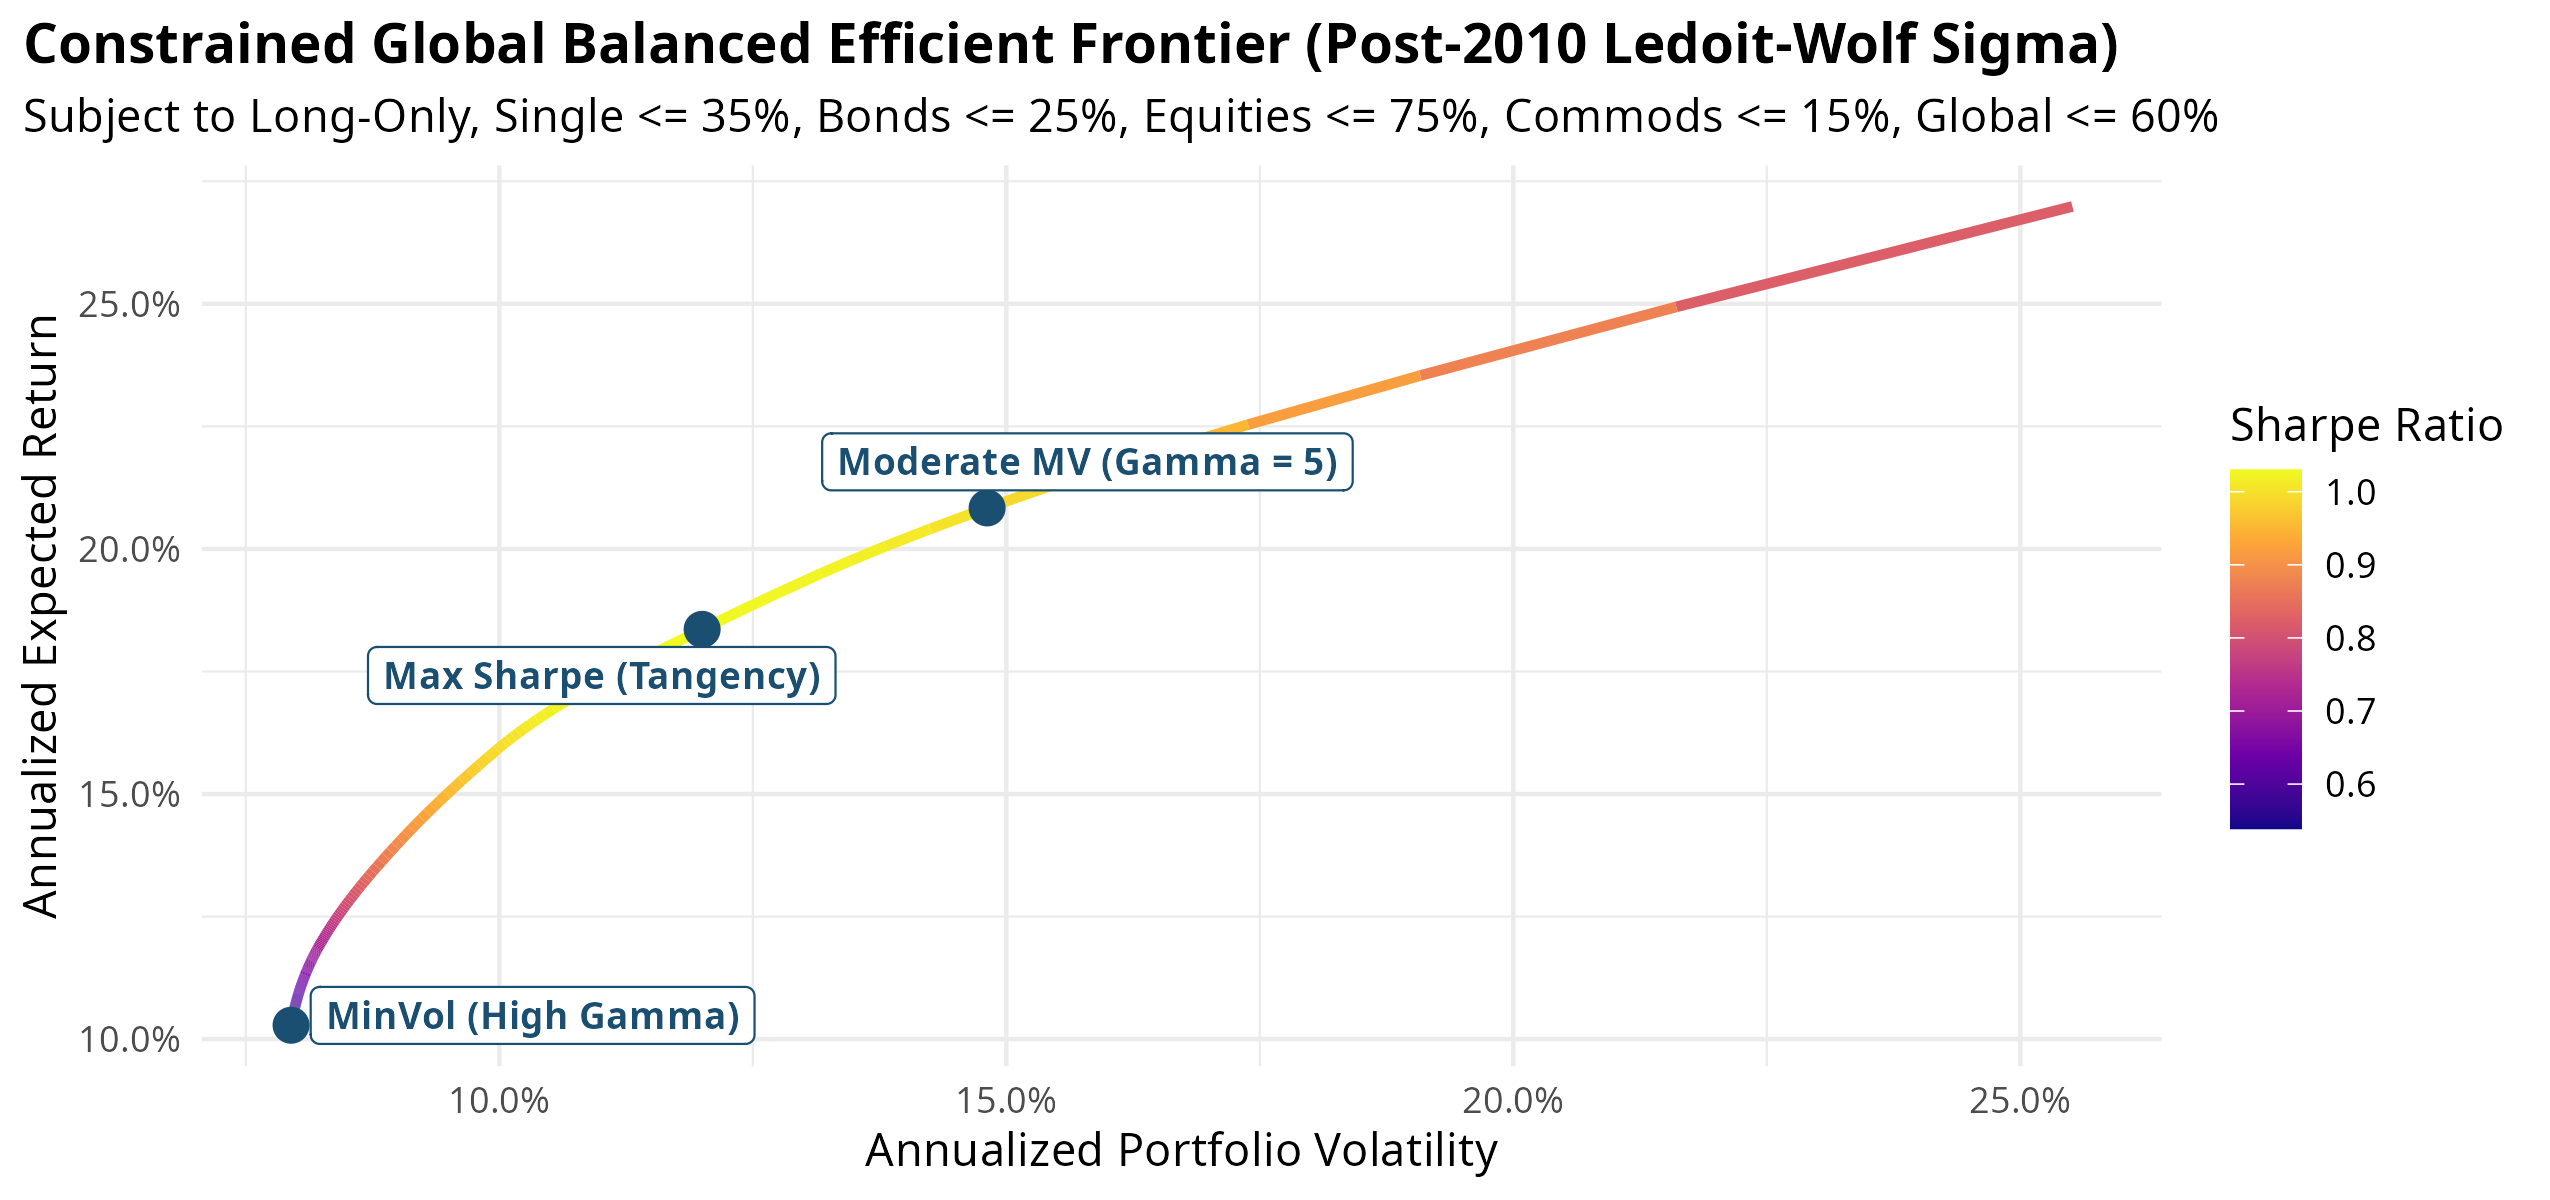
\includegraphics[width=1\linewidth]{figures/p_frontier} \caption{Efficient Frontier}\label{fig:p_frontier}
\end{figure}

\begin{table}[!h]
\centering
\caption{\label{tab:q4_static}Static Full-Sample Asset Class and Regional Allocations}
\centering
\begin{tabular}[t]{lrrrr}
\toprule
Allocation Bucket & MinVol & Max\_Sharpe & MV\_Gamma5 & ERC\\
\midrule
\addlinespace[0.3em]
\multicolumn{5}{l}{\textbf{Asset Class}}\\
\cellcolor{gray!10}{\hspace{1em}Bonds} & \cellcolor{gray!10}{25.0\%} & \cellcolor{gray!10}{25.0\%} & \cellcolor{gray!10}{10.0\%} & \cellcolor{gray!10}{28.6\%}\\
\hspace{1em}Commodities & 15.0\% & 15.0\% & 15.0\% & 13.3\%\\
\cellcolor{gray!10}{\hspace{1em}Equities} & \cellcolor{gray!10}{60.0\%} & \cellcolor{gray!10}{60.0\%} & \cellcolor{gray!10}{75.0\%} & \cellcolor{gray!10}{58.1\%}\\
\addlinespace[0.3em]
\multicolumn{5}{l}{\textbf{Region}}\\
\hspace{1em}Global & 60.0\% & 46.1\% & 60.0\% & 60.0\%\\
\cellcolor{gray!10}{\hspace{1em}Local} & \cellcolor{gray!10}{40.0\%} & \cellcolor{gray!10}{53.9\%} & \cellcolor{gray!10}{40.0\%} & \cellcolor{gray!10}{40.0\%}\\
\bottomrule
\end{tabular}
\end{table}

\section{Out-of-Sample Rolling Backtest and Turnover
Friction}\label{out-of-sample-rolling-backtest-and-turnover-friction}

Evaluating the strategies out-of-sample with quarterly rebalancing
(\(\ge 120\)-month expanding lookback) and 15 bps transaction costs
highlights a clear trade-off between return efficiency and trading
friction (Table \ref{tab:q4_oos_perf} and Figure
\ref{fig:p4_oos_wealth}). MV\_Gamma5 delivers the strongest
risk-adjusted performance with a 10.70\% net annualized return and 0.376
Net Sharpe ratio, outperforming Max\_Sharpe (9.84\% net return; 0.327
Sharpe) because stronger variance regularization curbs sensitivity to
noisy trailing sample means.However, return-seeking optimizers incur
substantial implementation drag: MV\_Gamma5 (20.30\% quarterly turnover)
and Max\_Sharpe (17.80\%) forfeit 6--10 bps annually to transaction
costs. By contrast, ERC achieves exceptional portfolio stability (4.06\%
quarterly turnover, preserving 8.68\% of its 8.69\% gross return), while
MinVol provides superior capital preservation with the lowest volatility
(11.50\%) and shallowest maximum drawdown (-23.80\%).

\begin{figure}[H]
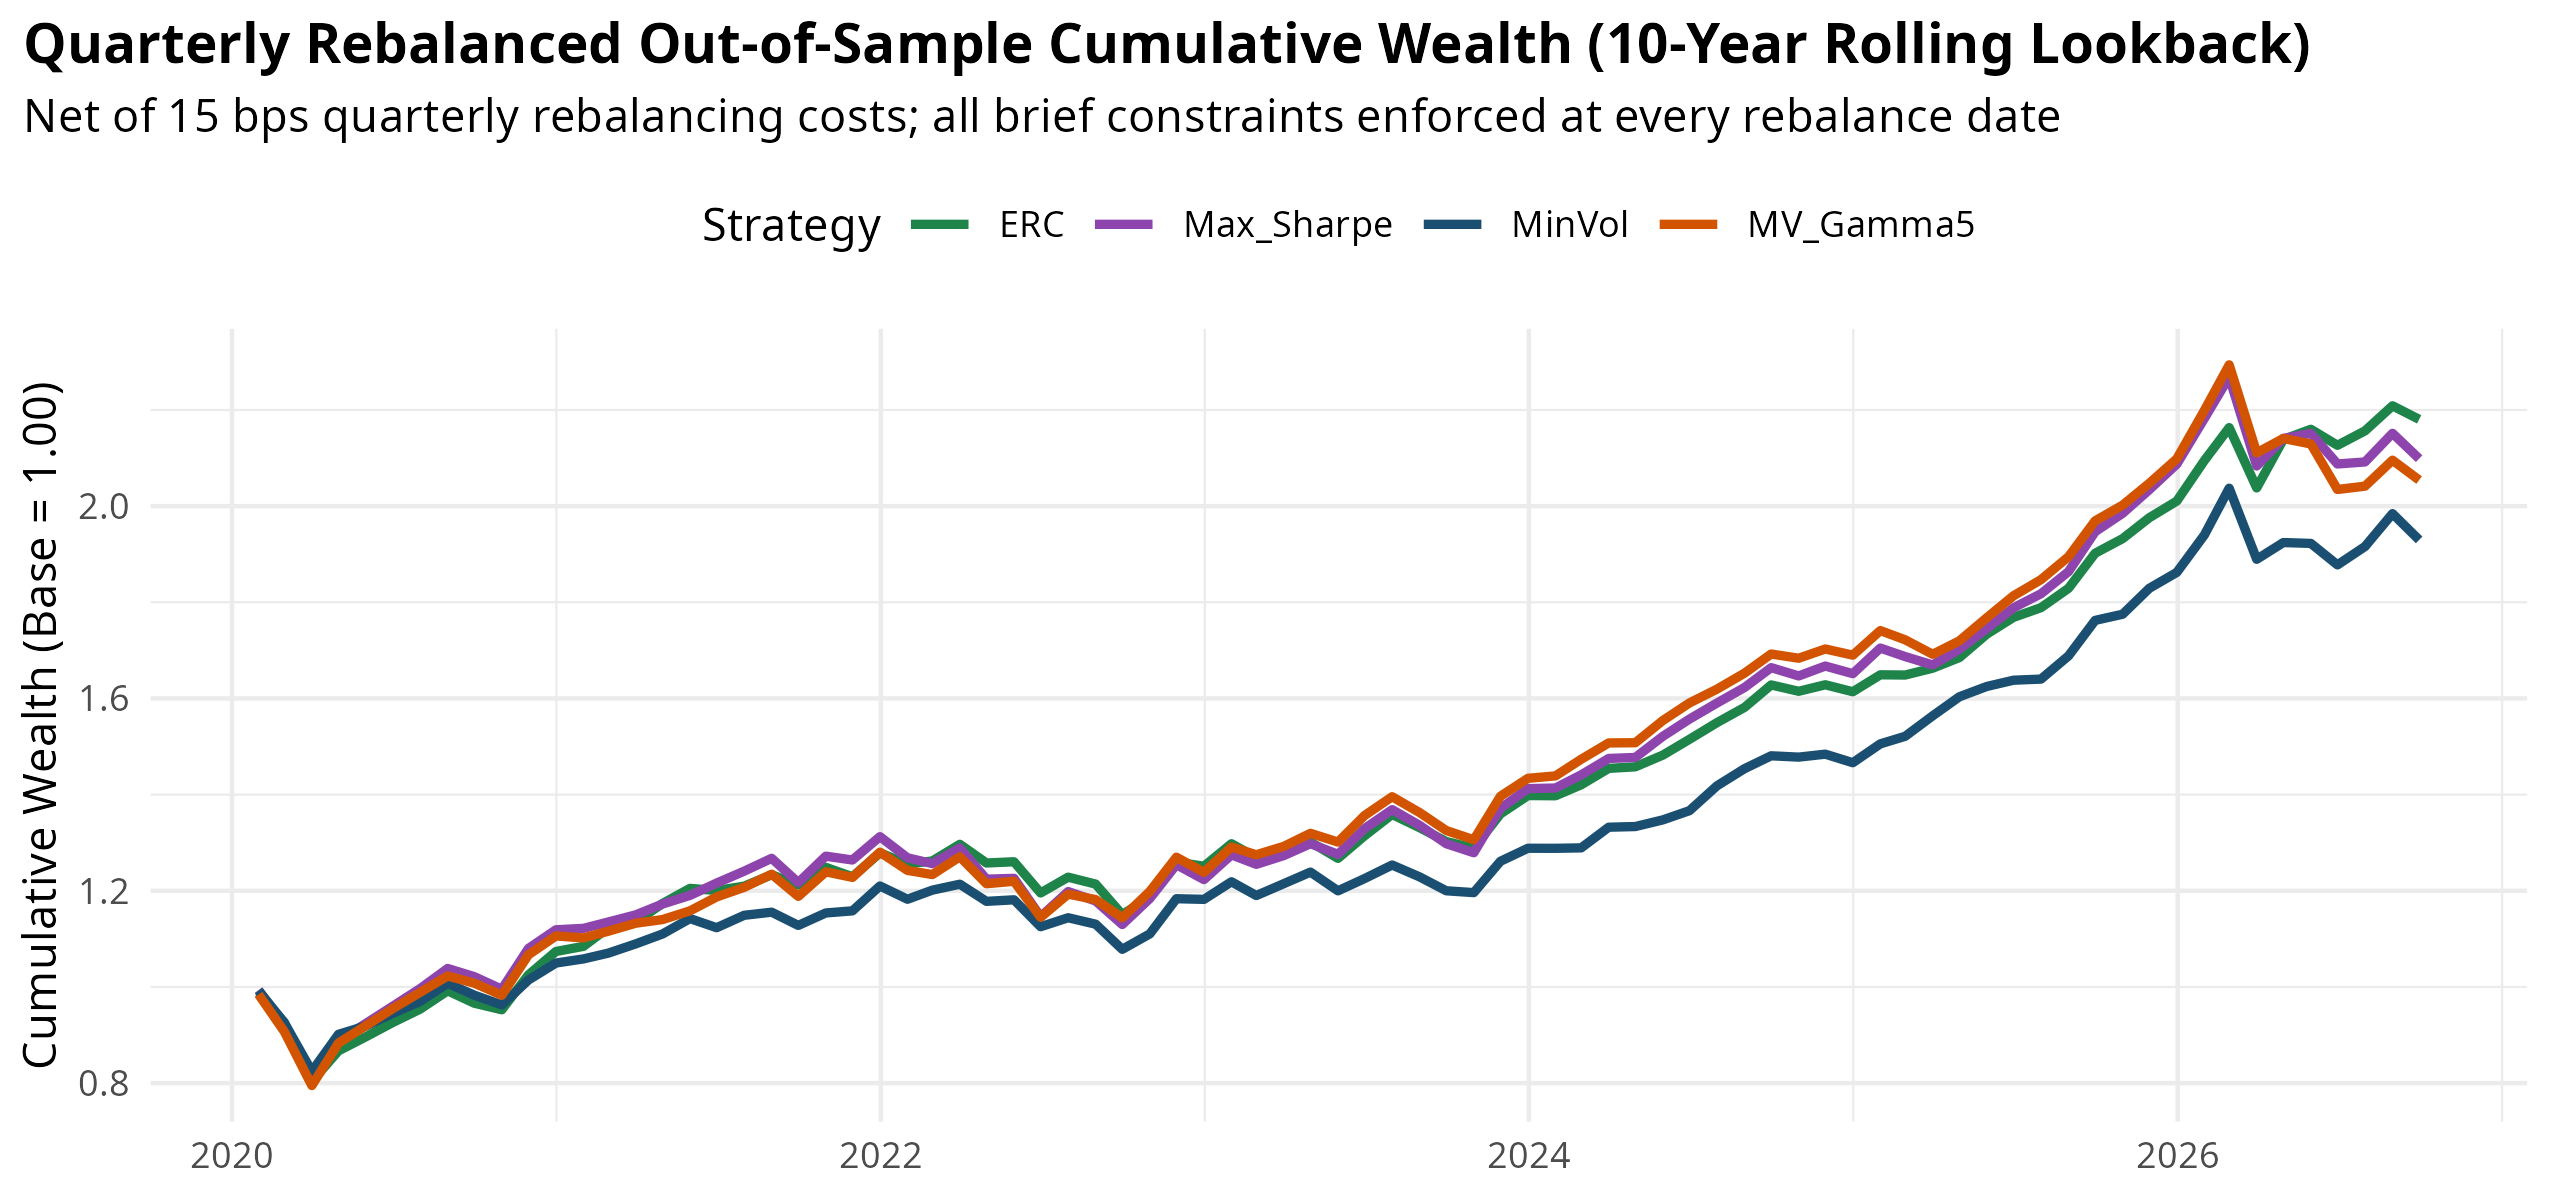
\includegraphics[width=1\linewidth]{figures/p_oos_wealth} \caption{oos wealth}\label{fig:p4_oos_wealth}
\end{figure}

\begin{table}[!h]
\centering
\caption{\label{tab:q4_oos_perf}Out-of-Sample Portfolio Performance Summary (Net of 15 bps Quarterly Rebalancing Costs)}
\centering
\begin{tabular}[t]{lrrrrrr}
\toprule
Strategy & Gross Ret. & Net Ret. & Ann. Vol. & Net Sharpe & Max DD & Avg. Qtr TO\\
\midrule
\cellcolor{gray!10}{ERC} & \cellcolor{gray!10}{8.69\%} & \cellcolor{gray!10}{8.68\%} & \cellcolor{gray!10}{12.07\%} & \cellcolor{gray!10}{0.256} & \cellcolor{gray!10}{28.29\%} & \cellcolor{gray!10}{4.06\%}\\
MV\_Gamma5 & 10.79\% & 10.71\% & 13.72\% & 0.376 & 27.61\% & 20.29\%\\
\cellcolor{gray!10}{Max\_Sharpe} & \cellcolor{gray!10}{9.90\%} & \cellcolor{gray!10}{9.84\%} & \cellcolor{gray!10}{13.11\%} & \cellcolor{gray!10}{0.327} & \cellcolor{gray!10}{28.76\%} & \cellcolor{gray!10}{17.77\%}\\
MinVol & 8.20\% & 8.17\% & 11.53\% & 0.221 & 23.84\% & 8.67\%\\
\bottomrule
\end{tabular}
\end{table}

\#Risk Budgeting and Macro Regime Stress Attribution Decomposing average
quarterly allocations into percentage variance contributions (Table
\ref{tab:q4_risk_budget} and Figure \ref{fig:q4-risk-comp}) exposes
significant risk concentration beneath seemingly balanced capital
weights. Even when MinVol and ERC hold roughly 58.5\%--60.3\% in
Equities, Equities still generate 70.4\%--72.4\% of total portfolio
variance. More striking is the hidden duration risk inside MV\_Gamma5:
its 25.9\% fixed-income allocation accounts for 43.2\% of total
portfolio risk due to heavy concentration in long-duration sovereign
bonds, while its near-zero Commodity weight (1.0\%) removes inflation
protection.

Macro regime attribution (Table \ref{tab:q4_regimes}) confirms how these
risk exposures behave under stress:

2020 COVID Shock: Sovereign bond rallies cushioned equity losses,
allowing Max\_Sharpe (-4.0\%) and MV\_Gamma5 (-4.5\%) to outperform ERC
(-7.4\%).

2022 Inflation \& Rate-Hiking Shock: Simultaneous equity and bond
sell-offs punished Max\_Sharpe (-6.8\%), whereas ERC (-2.2\%) and MinVol
(-2.3\%) proved far more resilient thanks to their 12.9\%--14.7\%
Commodity sleeves, before ERC led the subsequent recovery (+141.0\%).

\begin{table}[!h]
\centering
\caption{\label{tab:q4_risk_budget}Average Portfolio Weights and Percentage Risk Contributions by Asset Class}
\centering
\begin{tabular}[t]{lrrrrrrrr}
\toprule
\multicolumn{1}{c}{ } & \multicolumn{4}{c}{Average Weight} & \multicolumn{4}{c}{Risk Contribution} \\
\cmidrule(l{3pt}r{3pt}){2-5} \cmidrule(l{3pt}r{3pt}){6-9}
Asset Class & MinVol & MV5 & MaxSR & ERC & MinVol & MV5 & MaxSR & ERC\\
\midrule
\cellcolor{gray!10}{Bonds} & \cellcolor{gray!10}{25.0\%} & \cellcolor{gray!10}{25.9\%} & \cellcolor{gray!10}{25.7\%} & \cellcolor{gray!10}{28.6\%} & \cellcolor{gray!10}{11.4\%} & \cellcolor{gray!10}{43.2\%} & \cellcolor{gray!10}{27.1\%} & \cellcolor{gray!10}{18.1\%}\\
Commodities & 14.7\% & 1.0\% & 1.3\% & 12.9\% & 16.2\% & 0.3\% & 0.5\% & 11.5\%\\
\cellcolor{gray!10}{Equities} & \cellcolor{gray!10}{60.3\%} & \cellcolor{gray!10}{73.1\%} & \cellcolor{gray!10}{73.0\%} & \cellcolor{gray!10}{58.5\%} & \cellcolor{gray!10}{72.4\%} & \cellcolor{gray!10}{56.5\%} & \cellcolor{gray!10}{72.4\%} & \cellcolor{gray!10}{70.4\%}\\
\bottomrule
\end{tabular}
\end{table}

\begin{figure}[H]
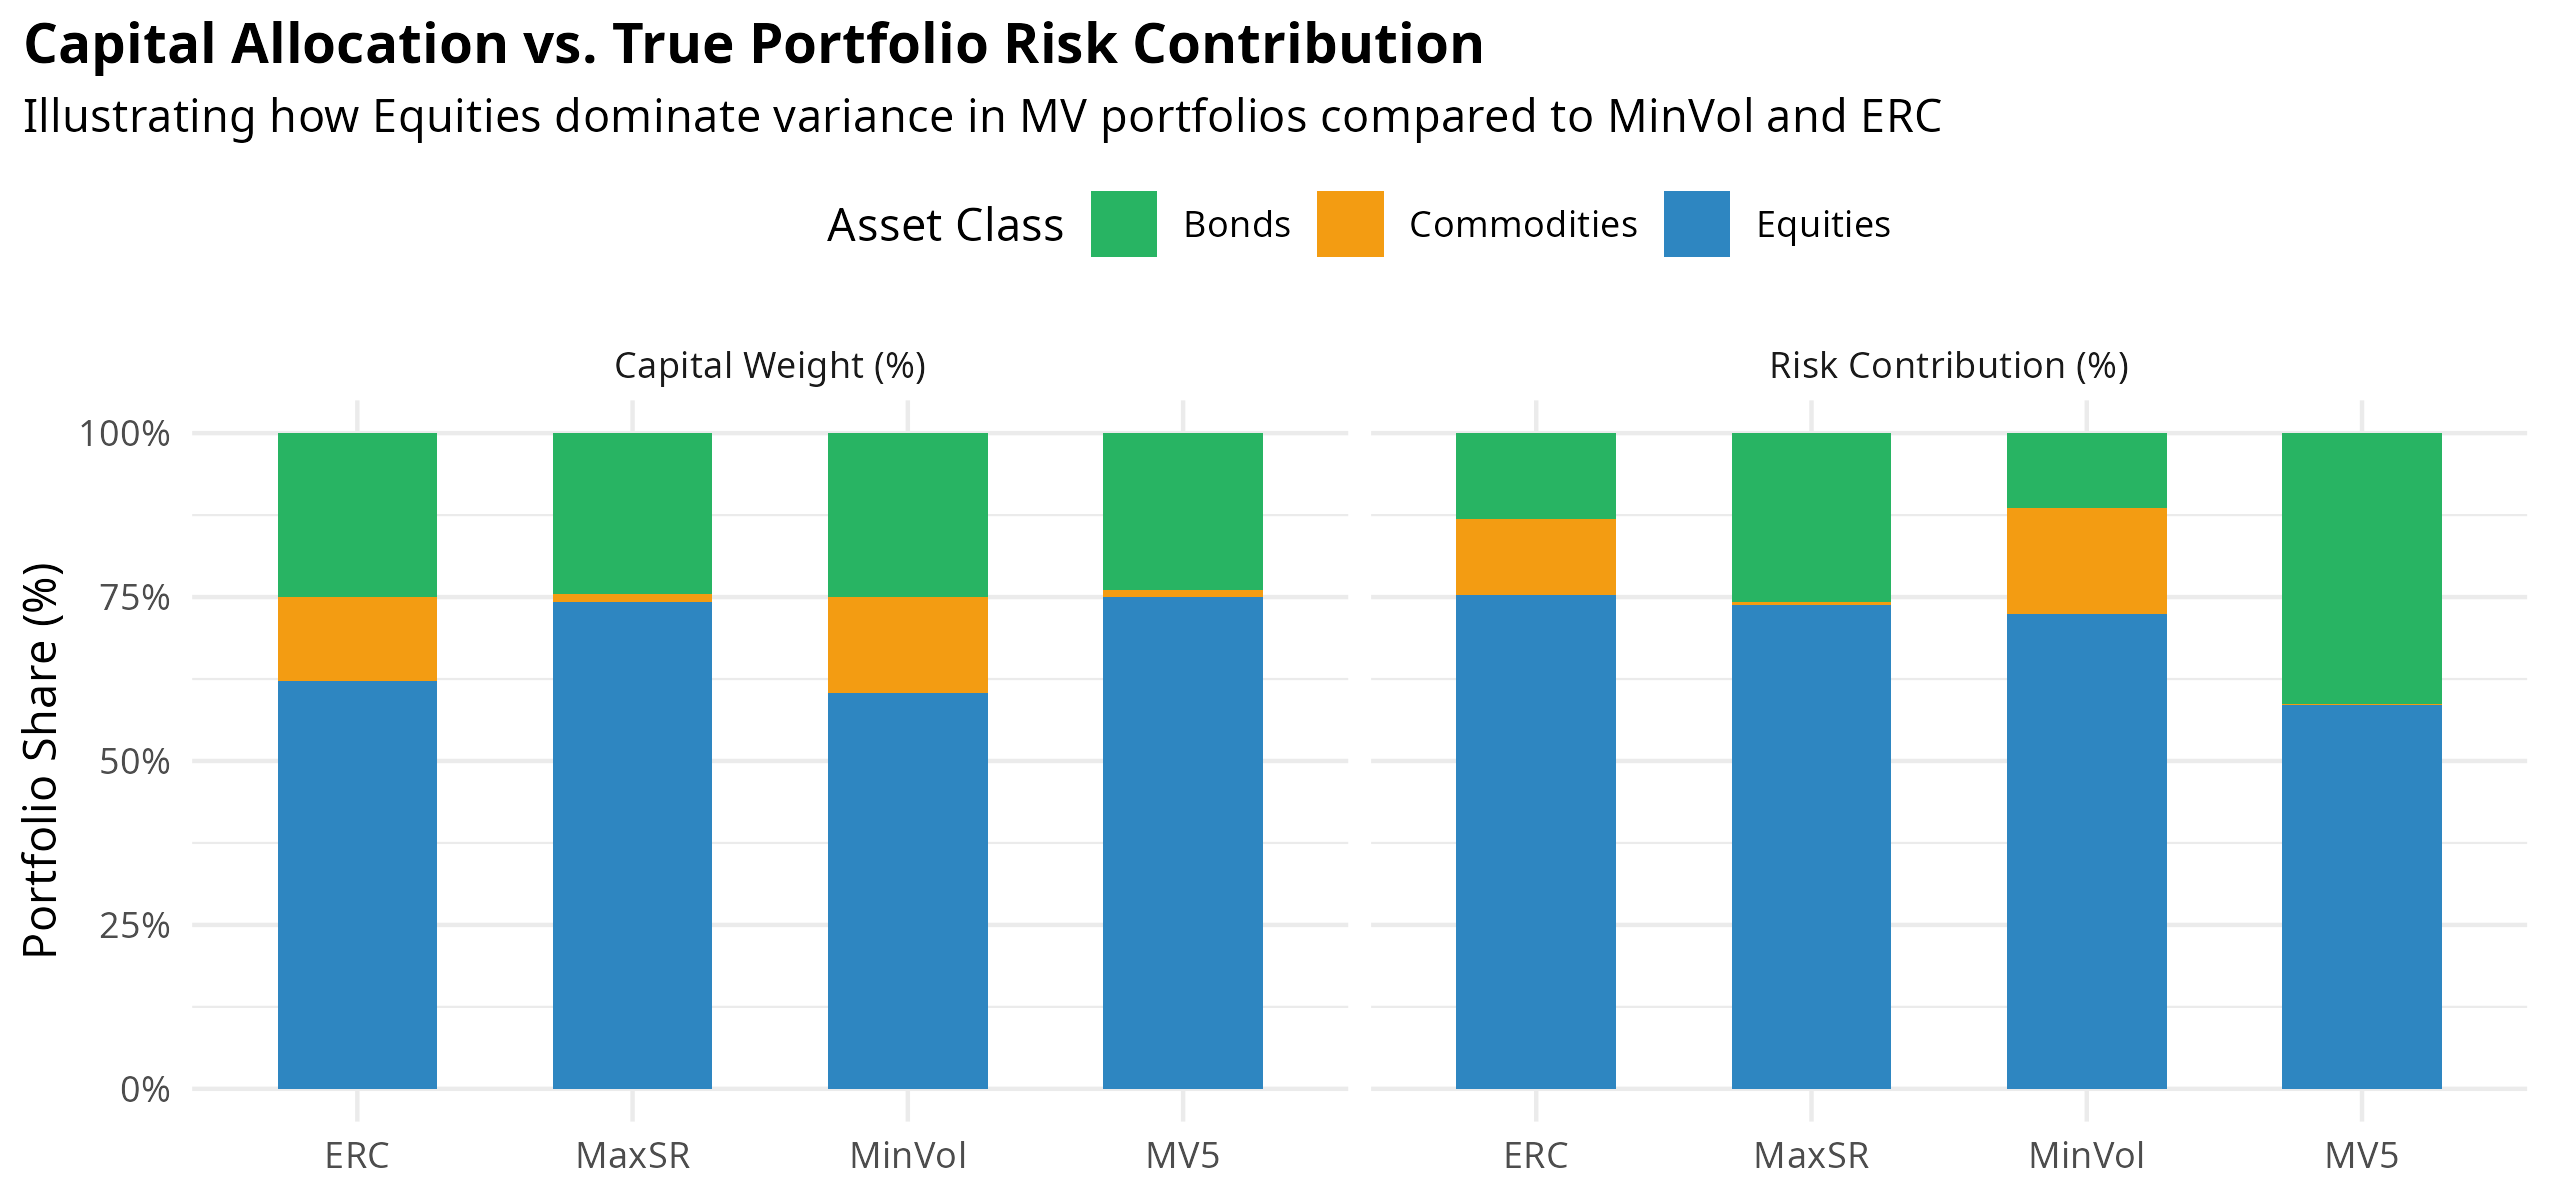
\includegraphics[width=1\linewidth]{figures/p_risk_comp} \caption{Risk comp}\label{fig:q4-risk-comp}
\end{figure}

\begin{table}[!h]
\centering
\caption{\label{tab:q4_regimes}Cumulative Strategy Returns Across Macro Regimes}
\centering
\begin{tabular}[t]{lrrrr}
\toprule
Market Regime & ERC & MV\_Gamma5 & Max\_Sharpe & MinVol\\
\midrule
\cellcolor{gray!10}{1. 2020 COVID Shock} & \cellcolor{gray!10}{-7.41\%} & \cellcolor{gray!10}{-4.53\%} & \cellcolor{gray!10}{-4.03\%} & \cellcolor{gray!10}{-5.51\%}\\
2. 2022 Inflation \& Rate Shock & -2.17\% & -3.27\% & -6.81\% & -2.30\%\\
\cellcolor{gray!10}{3. Recovery \& Normalization} & \cellcolor{gray!10}{140.73\%} & \cellcolor{gray!10}{122.44\%} & \cellcolor{gray!10}{134.64\%} & \cellcolor{gray!10}{109.04\%}\\
\bottomrule
\end{tabular}
\end{table}

\section{Conclusion}\label{conclusion}

Out-of-sample testing confirms a clear trade-off between return-seeking
mean-variance optimization and pure risk-based allocation: MV\_Gamma5
delivers the strongest risk-adjusted growth (10.70\% net annualized
return and a 0.376 Net Sharpe ratio), outperforming unregularized
tangency optimization (Max\_Sharpe, 0.327 Net Sharpe) by curbing
sensitivity to noisy sample return forecasts. Conversely, MinVol
provides superior capital preservation (11.50\% volatility and a
-23.80\% maximum drawdown), while ERC achieves exceptional portfolio
stability (4.06\% average quarterly turnover) and leads cumulative
performance during the post-2022 recovery (+141.0\%).

Furthermore, decomposing capital allocations into true variance
contributions reveals that nominal policy weights can obscure underlying
risk concentrations---most notably in MV\_Gamma5, where a 25.9\%
fixed-income allocation accounts for 43.2\% of portfolio risk, and where
near-zero Commodity exposure leaves the fund vulnerable during
inflationary rate shocks such as 2022. For an institutional mandate
prioritizing Sharpe maximization, MV\_Gamma5 is recommended; however,
for a balanced fiduciary mandate seeking smoother drawdowns, inflation
hedging, and minimal trading friction, a 50/50 strategic blend of
MV\_Gamma5 and ERC captures the upside of mean-variance optimization
while preserving the commodity ballast and low turnover of risk parity.
Future refinements could incorporate Bayes-Stein or Black-Litterman
expected-return shrinkage and explicit USD/ZAR currency-hedging overlays
to further stabilize offshore return attribution.

\bibliography{Tex/ref}





\end{document}
